\chapter{init Linux}
\section{Script de démarrage}
\subsection{Services}
\begin{itemize}
	\item sshd
	\item httpd
	\item ...
\end{itemize}

\section{Démons}
La liste des démons qui doivent être démarrés se trouve dans le fichier \textbf{/etc/inittab} qui décrit également quand et comment ils doivent être démarrés. Par exemple au démarrage du système, à l'arrêt du système, ...\\

Généralement les démons sont démarrés en mode \textbf{root}. Mais dans le programme du démon, on peut utiliser les appels systèmes \textbf{umask()}, \textbf{setsid()}, \textbf{setegid()} et \textbf{seteuid()} pour changer les droits du processus (démon) afin qu'il n'ait plus les droits \textbf{root} pour éviter qu'un attaquant puisse se servir du démon pour faire des choses en tant que \textbf{root}. \\

Dans ce la labo, le code source d'un démon était donné (daemon2.c). Il a fallu le compiler (\textbf{./buildroot/output/host/usr/bin/arm-linux-gnueabihf-gcc daemon2.c -o daemon2}
) pour la carte Odroid et copier l'exécutable sur la carte (directement dans \textbf{/home/}). \\

Ensuite il a fallu contrôler les droits du démon. Pour ce faire il à déjà fallu créer un utilisateur nommé \textbf{test} ainsi que le répertoire \textbf{/home/test/daemon/}.\\

Pour tester les droits, la première fois on a créé ce répertoire en tant qu'utilisateur \textbf{root}. Puis on à lancé le démon, et on a vérifié si il s'est exécuté correctement ou non avec le fichier \textbf{/var/log/messages}

\begin{center} 
\hspace{15cm}
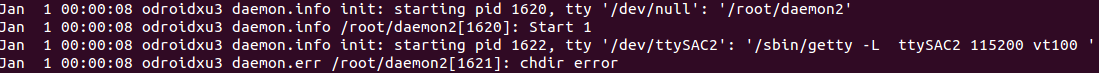
\includegraphics[width=16cm]{daemon_messages_1.png}
\end{center}
\vspace{0.5cm}

et la commande \textbf{ps -ale | grep daemon}

\begin{center} 
\hspace{15cm}
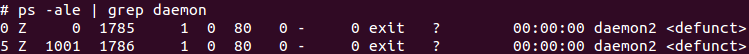
\includegraphics[width=16cm]{daemon_ps_1.png}
\end{center}
\vspace{0.5cm}

Cela nous a permis de constater que le démon n'a pas pu se lancer correctement (il n'est pas dans les processus en cours d'exécution) et que c'est parce qu'il n'a pas pu accéder au répertoire souhaité (\textbf{chdir error} indiqué dans le fichier \textbf{messages}, et si on regarde le code du démon, c'est qu'il n'a pas réussi à accéder au répertoire \textbf{/home/test/daemon}), probablement parce qu'il n'a pas les droits nécessaires.\\



\section{init kernel}
Avant start\_kernel, le processus init démarre les démons nécessaires. 

\section{runlevel}
\begin{lstlisting}[style=Bash]
# Startup the system
null::sysinit:/bin/mount -t proc proc /proc
null::sysinit:/bin/mount -o remount,rw /
null::sysinit:/bin/mkdir -p /dev/pts
null::sysinit:/bin/mkdir -p /dev/shm
null::sysinit:/bin/mount -a
null::sysinit:/bin/hostname -F /etc/hostname
# now run any rc scripts
::sysinit:/etc/init.d/rcS

# Put a getty on the serial port
ttySAC2::respawn:/sbin/getty -L  ttySAC2 115200 vt100 # GENERIC_SERIAL

# Stuff to do for the 3-finger salute
::ctrlaltdel:/sbin/reboot

# Stuff to do before rebooting
::shutdown:/etc/init.d/rcK
::shutdown:/sbin/swapoff -a
::shutdown:/bin/umount -a -r
\end{lstlisting}
Pas de runlevel sous Odroid

sysinit démarre avant toute autre commande telle que boot et bootwait.
